\documentclass[journal,compsoc]{IEEEtran}
\usepackage[utf8]{inputenc}
\usepackage{amsmath}
\usepackage{amssymb}
\usepackage{mathtools}
\usepackage{graphicx}
\usepackage{booktabs}
\usepackage{cite}
\usepackage{hyperref}
\usepackage{subcaption}
\usepackage{microtype}
\usepackage{tabularx}
\usepackage{amsthm}

\newtheorem{theorem}{Theorem}
\newtheorem{remark}{Remark}

\hypersetup{
    colorlinks=true,
    linkcolor=blue,
    citecolor=blue,
    urlcolor=blue
}

\begin{document}

\title{Adversarial Delay Amplification\\in Multi-Node Networks Under\\Timeout-Driven Retransmissions}

\author{Ilias~Chrysovergis%
\thanks{I.~Chrysovergis is with the Department of Electrical and Electronic Engineering, Imperial College London, London SW7 2AZ, UK, and Metatopia (e-mail: ilias@chrysovergis.gr).}}

\markboth{IEEE Networking Letters,~Vol.~XX, No.~X, Month~2026}%
{Chrysovergis: Adversarial Delay Amplification in Multi-Node Networks}

\maketitle

\begin{abstract}
We present a unified analytical framework for packet sojourn time in queueing networks under adversarial attacks and timeout-driven ARQ retransmissions. Using renewal-reward theory coupled with fixed-point traffic conservation, we analyze five progressively complex topologies: single-node destruction, single-node modification, $N$-node tandem chains, general feedforward networks, and symmetric feedback meshes. Key findings include a capacity divergence where modification attacks degrade throughput by $(1-p)^{-1}$ relative to destruction, super-linear delay growth in feedforward chains via hypoexponential moment-matching, and resilient delay scaling in meshes via Erlang visit summations. Simulations confirm all predictions within 2\% error.
\end{abstract}

\begin{IEEEkeywords}
Adversarial queueing, ARQ feedback loops, renewal-reward process, hypoexponential distribution, network delay analysis.
\end{IEEEkeywords}

\section{Introduction}
\IEEEPARstart{R}{eliable} data transport in tactical ad-hoc networks, autonomous swarms, and mission-critical IoT deployments relies on automatic repeat request (ARQ) retransmissions governed by timeout deadlines \cite{wood2002denial, pelechrinis2011denial, fall1996simulation}. In hostile environments, wireless channels are subject to active packet dropping (destruction) and payload tampering (modification). While retransmission mechanisms ensure eventual packet delivery, they induce an insidious \textit{positive feedback loop}:
\begin{align*}
\text{Adversarial Attacks} &\implies \text{Timeouts \& Retransmissions} \\
&\implies \text{Elevated Aggregate Load } \Lambda^* \\
&\implies \text{Longer Queueing Delays} \\
&\implies \text{Cascading Further Timeouts.}
\end{align*}
This feedback couples attack intensity, timeout deadlines, and queue dynamics, triggering severe delay amplification within nominal stability regions.

Yet prior queueing theory treats attacks and retransmissions largely in isolation: classical Jackson networks \cite{jackson1957networks} and $M/M/1$ queues \cite{kleinrock1975queueing} assume benign packet conservation, adversarial studies adopt fluid limits \cite{garetto2008modeling}, and G-networks with negative customers \cite{gelenbe1991product, gelenbe1993gnetworks} model packet deletion without end-to-end timeout cascades.

\begin{figure}[t]
    \centering
    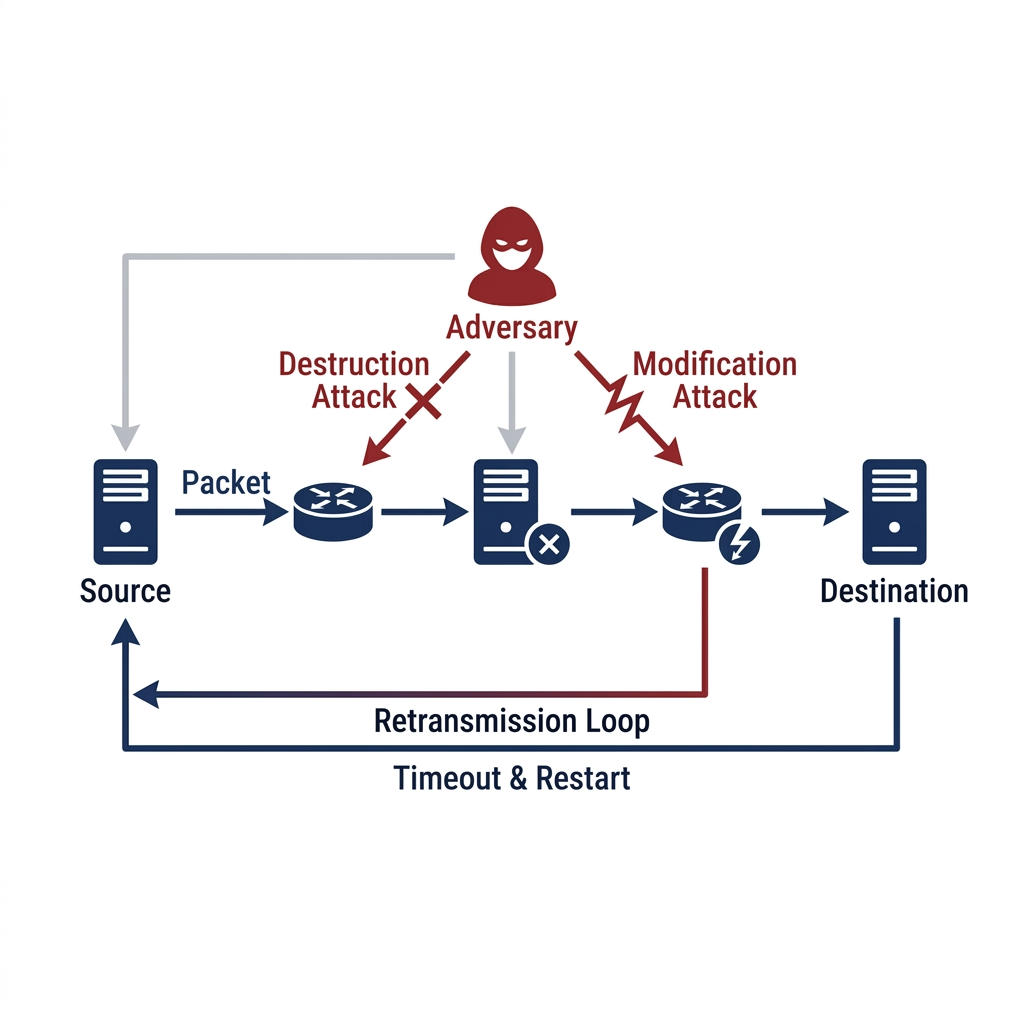
\includegraphics[width=0.32\textwidth]{fig1_system_model.png}
    \caption{Universal system model: External Poisson arrivals at rate $\lambda$ enter the network. Nodes serve packets at rate $\mu$. Adversaries attack packets with probability $p$. Attack losses or timeout expirations ($>W$) trigger origin-based retransmissions after backoff $B$, inducing an amplified traffic stream $\Lambda^*$.}
    \label{fig:model}
    \vspace{-4mm}
\end{figure}

This letter presents a unified analytical framework characterizing adversarial delay amplification across \textbf{five foundational case studies} of increasing topological complexity:
\begin{enumerate}
    \setlength{\itemsep}{0.5pt}
    \setlength{\parskip}{0pt}
    \item \textbf{Case 1: Single-Node Pre-Service Destruction} --- packets dropped pre-service; establishes baseline renewal-reward and fixed-point formulation.
    \item \textbf{Case 2: Single-Node Post-Service Modification} --- corruption detected post-service; reveals a $(1-p)^{-1}$ capacity penalty from wasted server cycles.
    \item \textbf{Case 3: Three-Node Tandem Chain} --- sequential forwarding under uniform load, yielding an exact Erlang-3 journey distribution.
    \item \textbf{Case 4: General $N$-Node Feedforward Network} --- stage attenuation $\Lambda_i^* = \Lambda_0^*(1-p)^i$, Hypoexponential moment-matching, and a 100\% stable operating envelope.
    \item \textbf{Case 5: Symmetric $N$-Node Feedback Mesh} --- Erlang-$k$ visit summations under Jackson routing, proving uniform load-balancing prevents bottlenecking.
\end{enumerate}
All five models are validated via SimPy simulations \cite{matloff2008introduction} with errors below 2\% overall and under 0.65\% for multi-node topologies.

\section{Universal Renewal-Reward Framework}
Consider a queueing network with external Poisson arrivals at rate $\lambda$ (Fig.~\ref{fig:model}). Each packet undergoes a sequence of independent and identically distributed (i.i.d.) transmission attempts until successful delivery. An adversary corrupts or destroys each attempt independently with probability $p$. A global timeout window $W$ aborts any attempt whose cumulative delay exceeds $W$. Failed packets are retransmitted from the origin after a deterministic backoff $B \ge 0$.

Let $P_{\text{succ}}$ denote the probability that an attempt succeeds (survives attacks and completes within $W$). The total attempt count $A$ is geometrically distributed: $P(A = a) = (1 - P_{\text{succ}})^{a-1} P_{\text{succ}}$ for $a \ge 1$, with expectation $E[A] = 1/P_{\text{succ}}$. Each packet incurs $A - 1$ failed attempts followed by exactly one successful attempt. Applying the renewal-reward theorem \cite{ross1996stochastic}, the mean end-to-end sojourn time $E[D]$ is:
\begin{equation}
E[D] = (E[A] - 1)\, E[D_{\text{fail}}] + E[D_{\text{succ}}] + (E[A] - 1)\, B
\label{eq:renewal}
\end{equation}
where $E[D_{\text{fail}}]$ and $E[D_{\text{succ}}]$ are the conditional expected durations of failed and successful attempts, respectively.

Because every failed attempt generates a retransmission, the total arrival rate $\Lambda^*$ entering the network exceeds the external arrival rate $\lambda$. By flow conservation:
\begin{equation}
\Lambda^* = \lambda \cdot E[A] = \frac{\lambda}{P_{\text{succ}}(\Lambda^*)}
\label{eq:fixed_point}
\end{equation}
Equation~\eqref{eq:fixed_point} is a non-linear fixed-point equation. Because queueing delays increase monotonically with $\Lambda^*$, the success probability $P_{\text{succ}}(\Lambda^*)$ is monotonically decreasing in $\Lambda^*$. A stable steady-state exists if and only if \eqref{eq:fixed_point} admits a unique root satisfying the topology-specific bottleneck stability criterion: $\Lambda^* < \Lambda_{\text{crit}}$.

\section{Single-Node Topologies (Cases 1 \& 2)}
Consider an isolated $M/M/1$ queue with service rate $\mu$, timeout $W$, and attack probability $p$.

\subsection{Case 1: Pre-Service Destruction Attacks}
In destruction attacks, the adversary intercepts packets at the queue head prior to service. Attacked packets exit without consuming server processing time. Only surviving packets enter the server, so the effective service load is $\lambda_{\text{eff}} = \Lambda^*(1 - p) \implies \rho = \Lambda^*(1 - p)/\mu < 1$. The system operates as an $M/M/1$ queue with arrival rate $\lambda_{\text{eff}}$. The cumulative distribution of total time in system (waiting $W_q$ plus service $S$) is $P(W_q + S \le t) = 1 - \rho e^{-(\mu - \lambda_{\text{eff}})t}$. An attempt succeeds if it escapes attack and completes before timeout $W$:
\begin{equation}
P_{\text{succ}} = (1 - p)\!\left[1 - \frac{\Lambda^*(1\!-\!p)}{\mu}\, e^{-(\mu - \Lambda^*(1-p))W}\right]
\label{eq:psucc_destr}
\end{equation}
The expected delay per attempt comprises queue waiting plus conditional service: $E[D_{\text{attempt}}] = E[W_q] + (1-p)/\mu$. Substituting into \eqref{eq:renewal}:
\begin{equation}
E[D] = \frac{1}{P_{\text{succ}}}\!\left[\frac{\Lambda^*(1\!-\!p)}{\mu(\mu - \Lambda^*(1\!-\!p))} + \frac{1\!-\!p}{\mu}\right] + \left(\frac{1}{P_{\text{succ}}} - 1\right)\!B
\label{eq:delay_destr}
\end{equation}
Stability requires $\Lambda^*(1-p) < \mu \implies \Lambda^* < \mu/(1-p)$.

\subsection{Case 2: Post-Service Modification Attacks}
In modification attacks, the adversary tampers with packet payloads during transmission. Integrity violations are detected via checksums only \textit{after} full service completion ($S \sim \text{Exp}(\mu)$). Hence, every attempt—successful or corrupted—occupies the server for a full service interval. The arrival rate at the server is the unattenuated rate $\Lambda^*$, yielding utilization $\rho = \Lambda^* / \mu$. The total duration per attempt follows $S \sim \text{Exp}(\mu - \Lambda^*)$ with CDF $P(S \le t) = 1 - e^{-(\mu - \Lambda^*)t}$. Success requires escaping attack and completing within $W$:
\begin{equation}
P_{\text{succ}} = (1 - p)\left(1 - e^{-(\mu - \Lambda^*)W}\right)
\label{eq:psucc_mod}
\end{equation}
Since all attempts consume an average of $E[S] = (\mu - \Lambda^*)^{-1}$, the mean sojourn time simplifies to:
\begin{equation}
E[D] = \frac{1}{(1 - p)\left(1 - e^{-(\mu - \Lambda^*)W}\right)(\mu - \Lambda^*)}
\label{eq:delay_mod}
\end{equation}
Stability requires $\Lambda^* < \mu$, which bounds the external arrival rate by $\lambda < \mu(1-p)(1 - e^{-\mu W})$.

\begin{figure}[t]
    \centering
    \begin{subfigure}[b]{0.23\textwidth}
        
\includegraphics[width=\textwidth]{destroy_no_service_plot_reps200.png}
        \caption{Case 1: Destruction}
    \end{subfigure}
    \hfill
    \begin{subfigure}[b]{0.23\textwidth}
        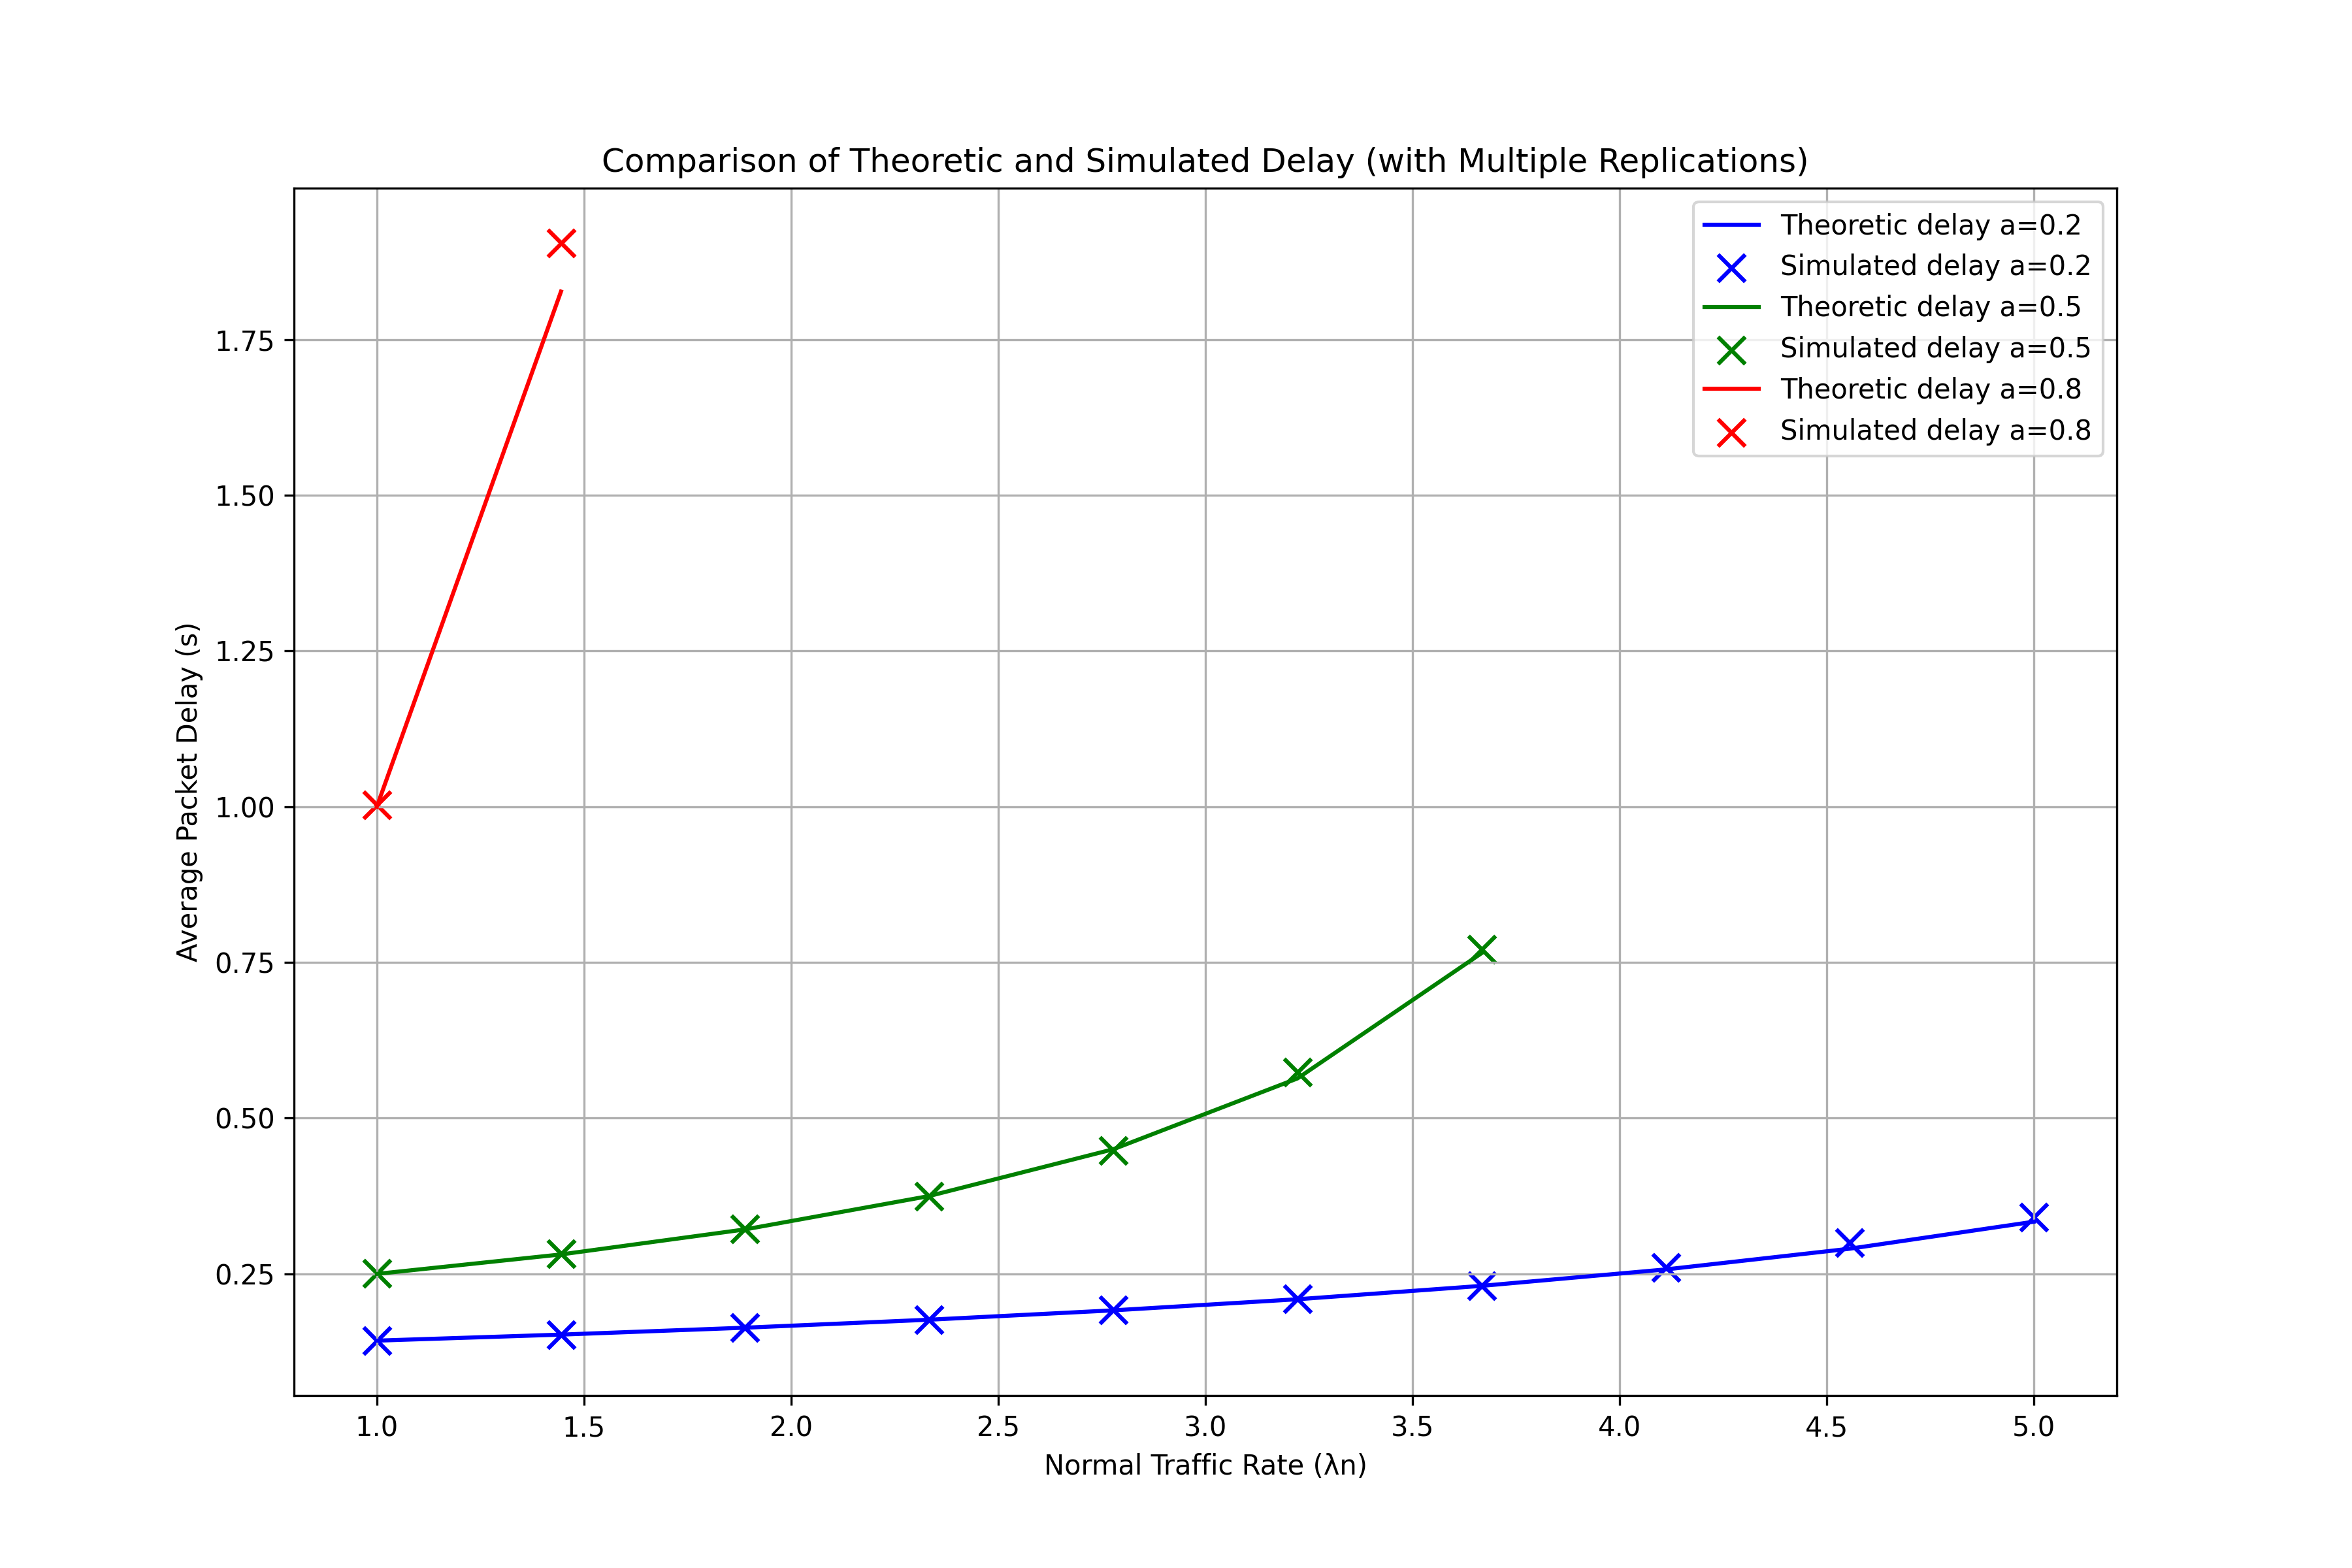
\includegraphics[width=\textwidth]{plot_reps50_warmup500_sim5000.png}
        \caption{Case 2: Modification}
    \end{subfigure}
    \caption{Single-node expected delay vs.\ arrival rate $\lambda$. Modification attacks cause substantially earlier queue saturation due to wasted service cycles. Solid lines: theoretical model; markers: SimPy simulation results.}
    \label{fig:single}
    \vspace{-3mm}
\end{figure}

\begin{theorem}[Capacity Divergence]
Let $\Lambda_{\emph{crit}}^{\emph{dest}}$ and $\Lambda_{\emph{crit}}^{\emph{mod}}$ denote the critical saturation capacities under pre-service destruction and post-service modification attacks. Then $\Lambda_{\emph{crit}}^{\emph{dest}} / \Lambda_{\emph{crit}}^{\emph{mod}} = (1 - p)^{-1}$. Post-service modification degrades sustainable system throughput by an exact factor of $(1-p)^{-1}$ relative to pre-service destruction. At $p = 0.5$, modification attacks halve the sustainable throughput (Fig.~\ref{fig:single}).
\end{theorem}

\section{Feedforward Network Topologies (Cases 3 \& 4)}

\subsection{Hypoexponential Journey Time \& Burke's Theorem}
Consider an $N$-node tandem chain ($0 \to 1 \to \cdots \to N\!-\!1$) where each node has service rate $\mu$. By Burke's theorem \cite{burke1956output}, in steady state the departure process of an $M/M/1$ queue is Poisson. Hence, each intermediate node $i$ operates as an independent $M/M/1$ queue with sojourn time $X_i \sim \text{Exp}(\mu - \Lambda_i^*)$, with mean $T_i = (\mu - \Lambda_i^*)^{-1}$ and variance $T_i^2$.

The cumulative journey time across all $N$ stages is the sum of $N$ independent exponential stages with distinct rates: $S_N = \sum_{i=0}^{N-1} X_i \sim \text{Hypoexponential}(\mu - \Lambda_0^*, \dots, \mu - \Lambda_{N-1}^*)$. Because the exact Hypoexponential CDF involves alternating convolution sums that become numerically ill-conditioned for large $N$, we employ a robust two-parameter Gamma moment-matching approximation \cite{altiok1985approximate, cox1955use}: $S_N \sim \text{Gamma}(k, \theta)$ with:
\begin{equation}
k = \frac{\mu_S^2}{\sigma_S^2} = \frac{\left(\sum_{i=0}^{N-1} T_i\right)^2}{\sum_{i=0}^{N-1} T_i^2}, \quad \theta = \frac{\sigma_S^2}{\mu_S} = \frac{\sum_{i=0}^{N-1} T_i^2}{\sum_{i=0}^{N-1} T_i}
\label{eq:gamma_moments}
\end{equation}
The timeout-free probability is $p_{\text{no\_to}} = P(S_N \le W) = \frac{\gamma(k, W/\theta)}{\Gamma(k)}$, where $\gamma(s, x) = \int_0^x t^{s-1} e^{-t} dt$ is the lower incomplete gamma function.

\subsection{Case 3: Three-Node Tandem Chain ($N=3$)}
When node arrival rates are identical ($\Lambda_0^* = \Lambda_1^* = \Lambda_2^* = \Lambda^*$), journey statistics simplify to $\mu_S = 3/(\mu - \Lambda^*)$ and $\sigma_S^2 = 3/(\mu - \Lambda^*)^2$. Hence $k = 3$ and $\theta = (\mu - \Lambda^*)^{-1}$, reducing $S_3$ to an exact Erlang-3 distribution:
\begin{align}
P_{\text{succ}} &= (1 - p)^3 \left[1 - \sum_{m=0}^2 \frac{[(\mu - \Lambda^*)W]^m e^{-(\mu - \Lambda^*)W}}{m!}\right] \\
E[D] &= \frac{3}{P_{\text{succ}}(\mu - \Lambda^*)}
\end{align}

\subsection{Case 4: General $N$-Node Feedforward Networks}
In a general $N$-node chain with stage attack probability $p$, packets attacked at stage $i$ drop out and do not proceed to stage $i+1$. Traffic attenuates geometrically: $\Lambda_i^* = \Lambda_0^* (1 - p)^i$ for $i \in \{0, \dots, N-1\}$. Stage sojourn times are $T_i = [\mu - \Lambda_0^*(1-p)^i]^{-1}$. Overall success requires surviving all $N$ stages and completing within timeout $W$:
\begin{equation}
P_{\text{succ}} = (1 - p)^N \frac{\gamma(k, W/\theta)}{\Gamma(k)}
\label{eq:psucc_ff}
\end{equation}

Conditional expectations for successful and failed attempts are:
\begin{enumerate}
    \setlength{\itemsep}{1pt}
    \item \textbf{Successful Attempt Duration:} Using truncated Gamma moments:
    \begin{equation}
    E[D_{\text{succ}}] = E[S_N \mid S_N \le W] = \mu_S \frac{\gamma(k+1, W/\theta)}{\gamma(k, W/\theta)}
    \label{eq:trunc_succ}
    \end{equation}
    \item \textbf{Failed Attempt Duration:} Failures arise from two disjoint events: (i) an attack at stage $i$ (probability $(1-p)^i p$) with duration $\sum_{j=0}^i T_j$, or (ii) an end-to-end timeout after surviving all stages (probability $(1-p)^N (1 - p_{\text{no\_to}})$) with duration $E[S_N \mid S_N > W] = \mu_S \frac{1 - \gamma(k+1, W/\theta)/\Gamma(k+1)}{1 - \gamma(k, W/\theta)/\Gamma(k)}$:
    \begin{align}
    E[D_{\text{fail}}] &= \frac{1}{1 - P_{\text{succ}}} \Bigg[\sum_{i=0}^{N-1} (1-p)^i p \sum_{j=0}^i T_j \nonumber \\
    &\quad + (1-p)^N (1 - p_{\text{no\_to}})\, E[S_N \mid S_N > W]\Bigg]
    \label{eq:delay_fail_ff}
    \end{align}
\end{enumerate}
Total delay is $E[D] = (P_{\text{succ}}^{-1} - 1) E[D_{\text{fail}}] + E[D_{\text{succ}}]$.

\begin{figure}[t]
    \centering
    \begin{subfigure}[b]{0.23\textwidth}
        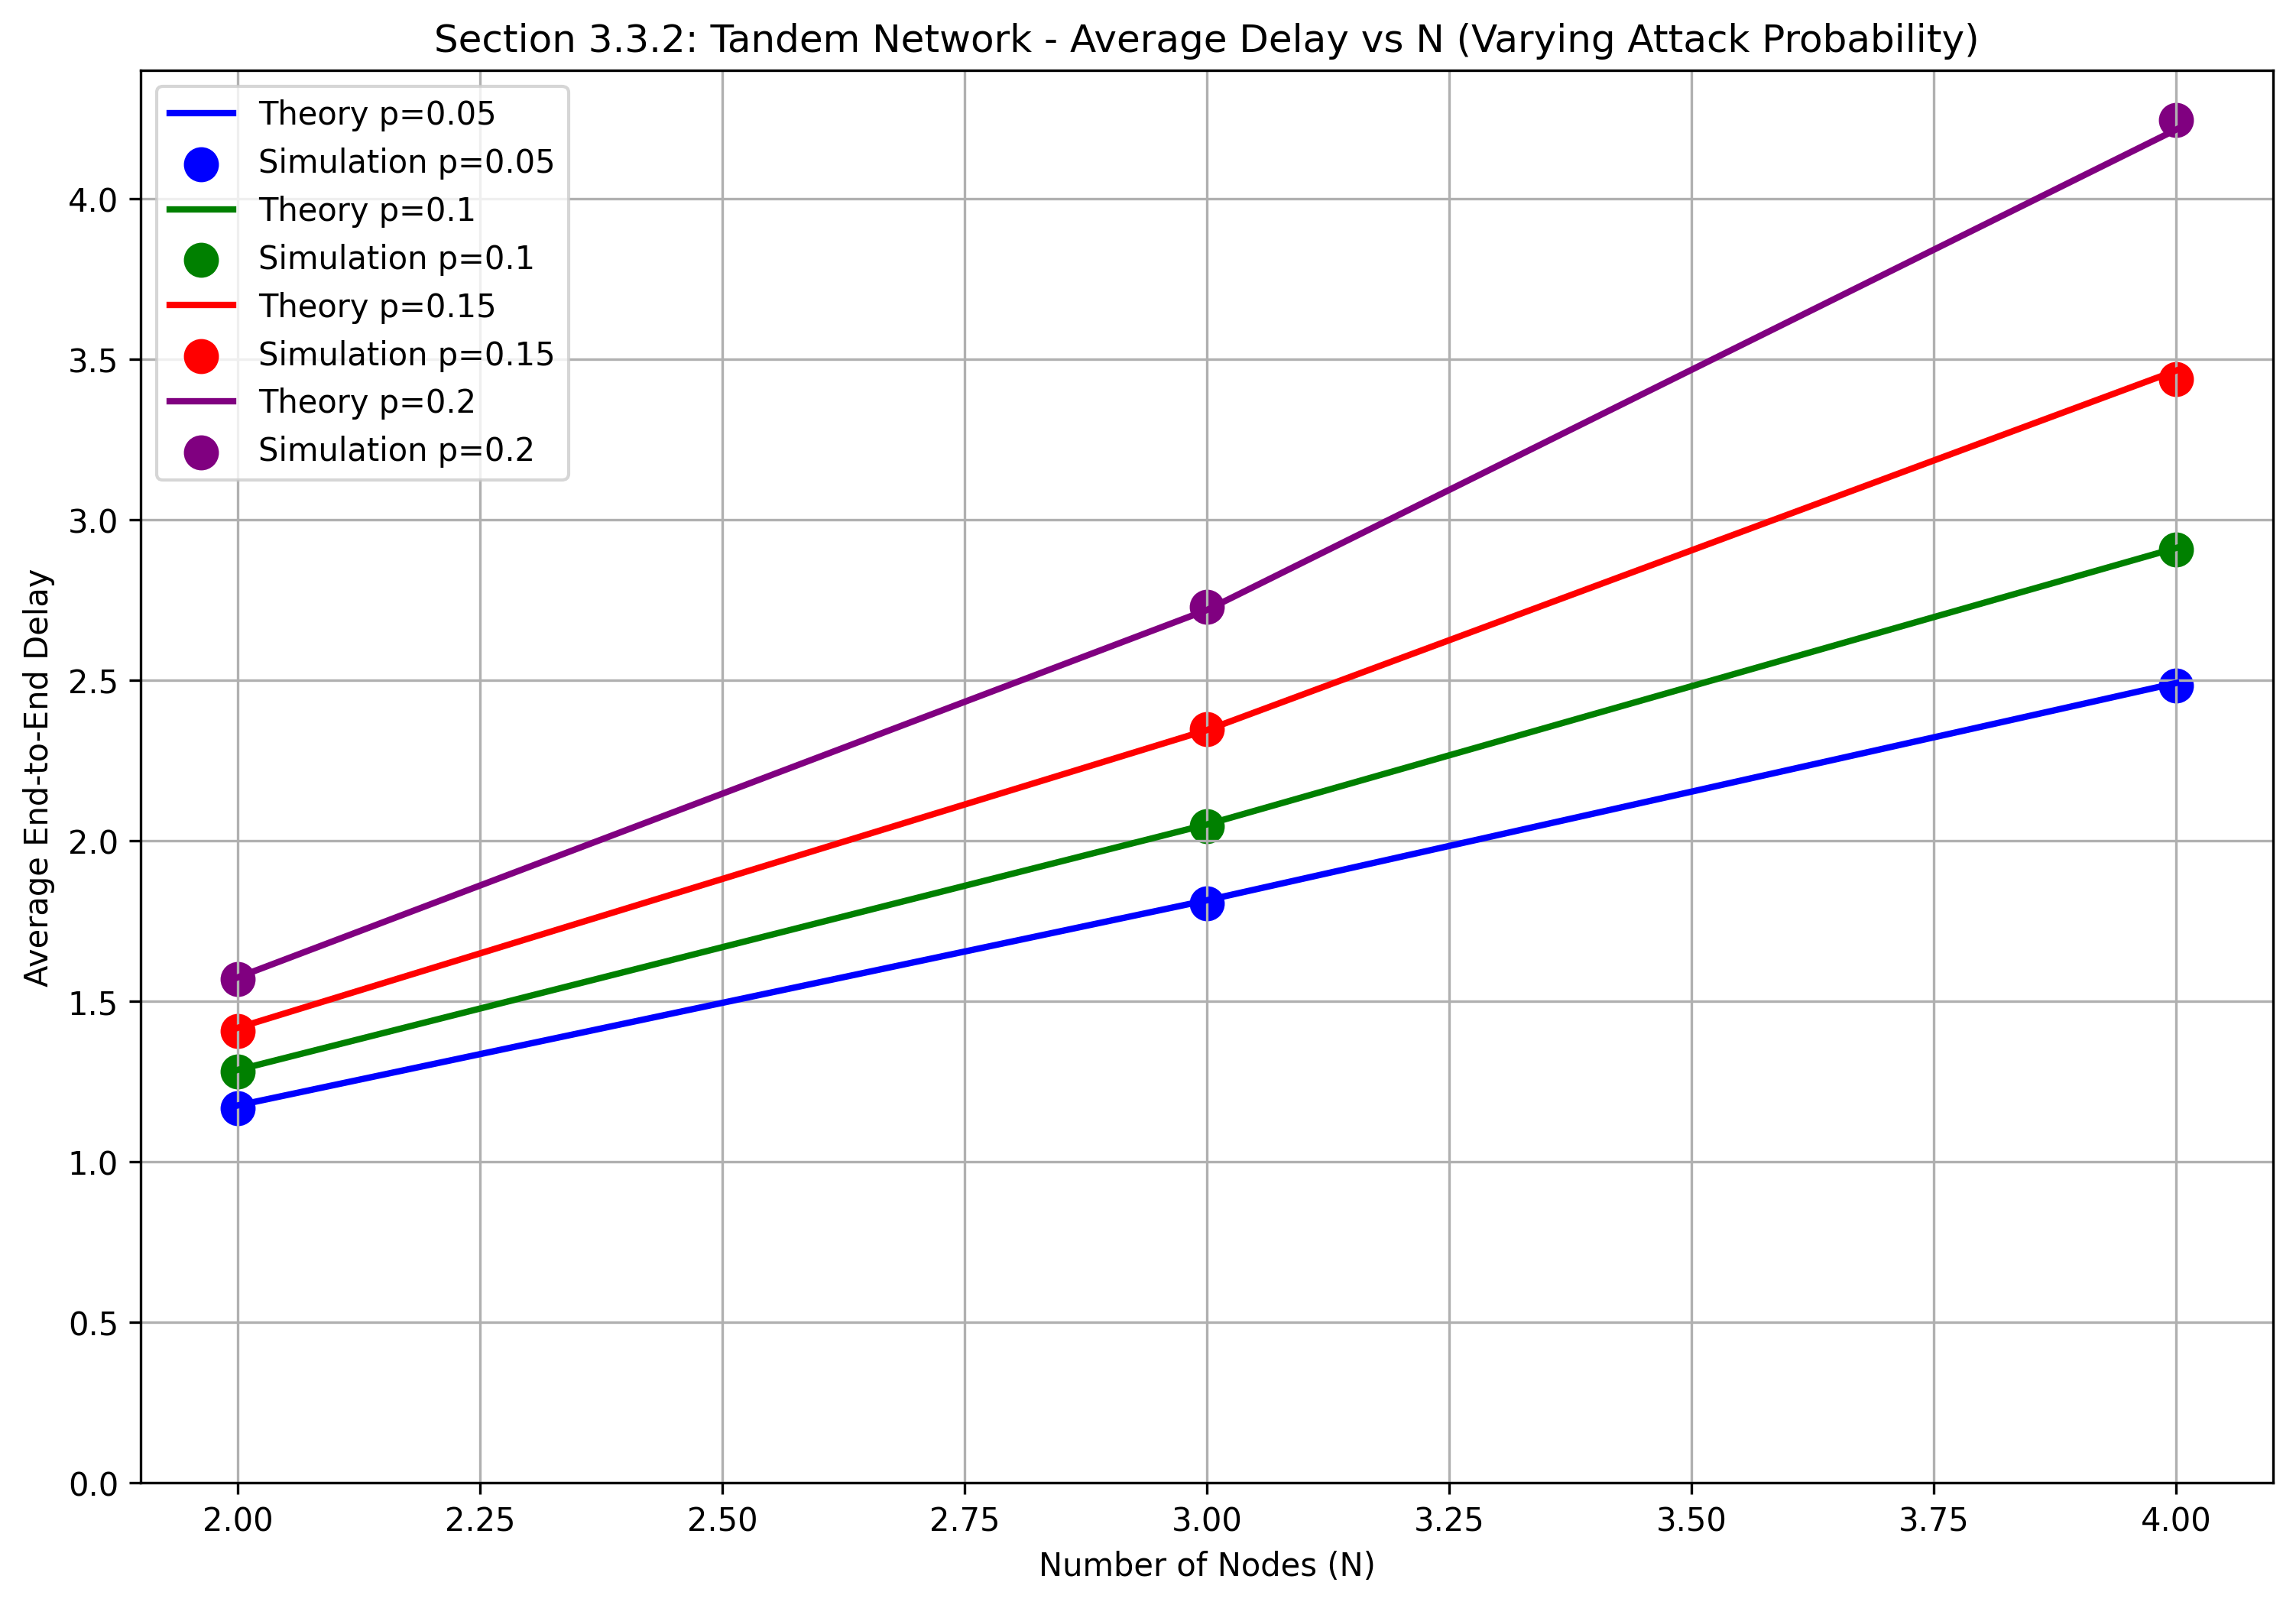
\includegraphics[width=\textwidth]{section_3_3_2_tandem_delay_vs_N_varying_p.png}
        \caption{Delay vs.\ chain length $N$}
    \end{subfigure}
    \hfill
    \begin{subfigure}[b]{0.23\textwidth}
        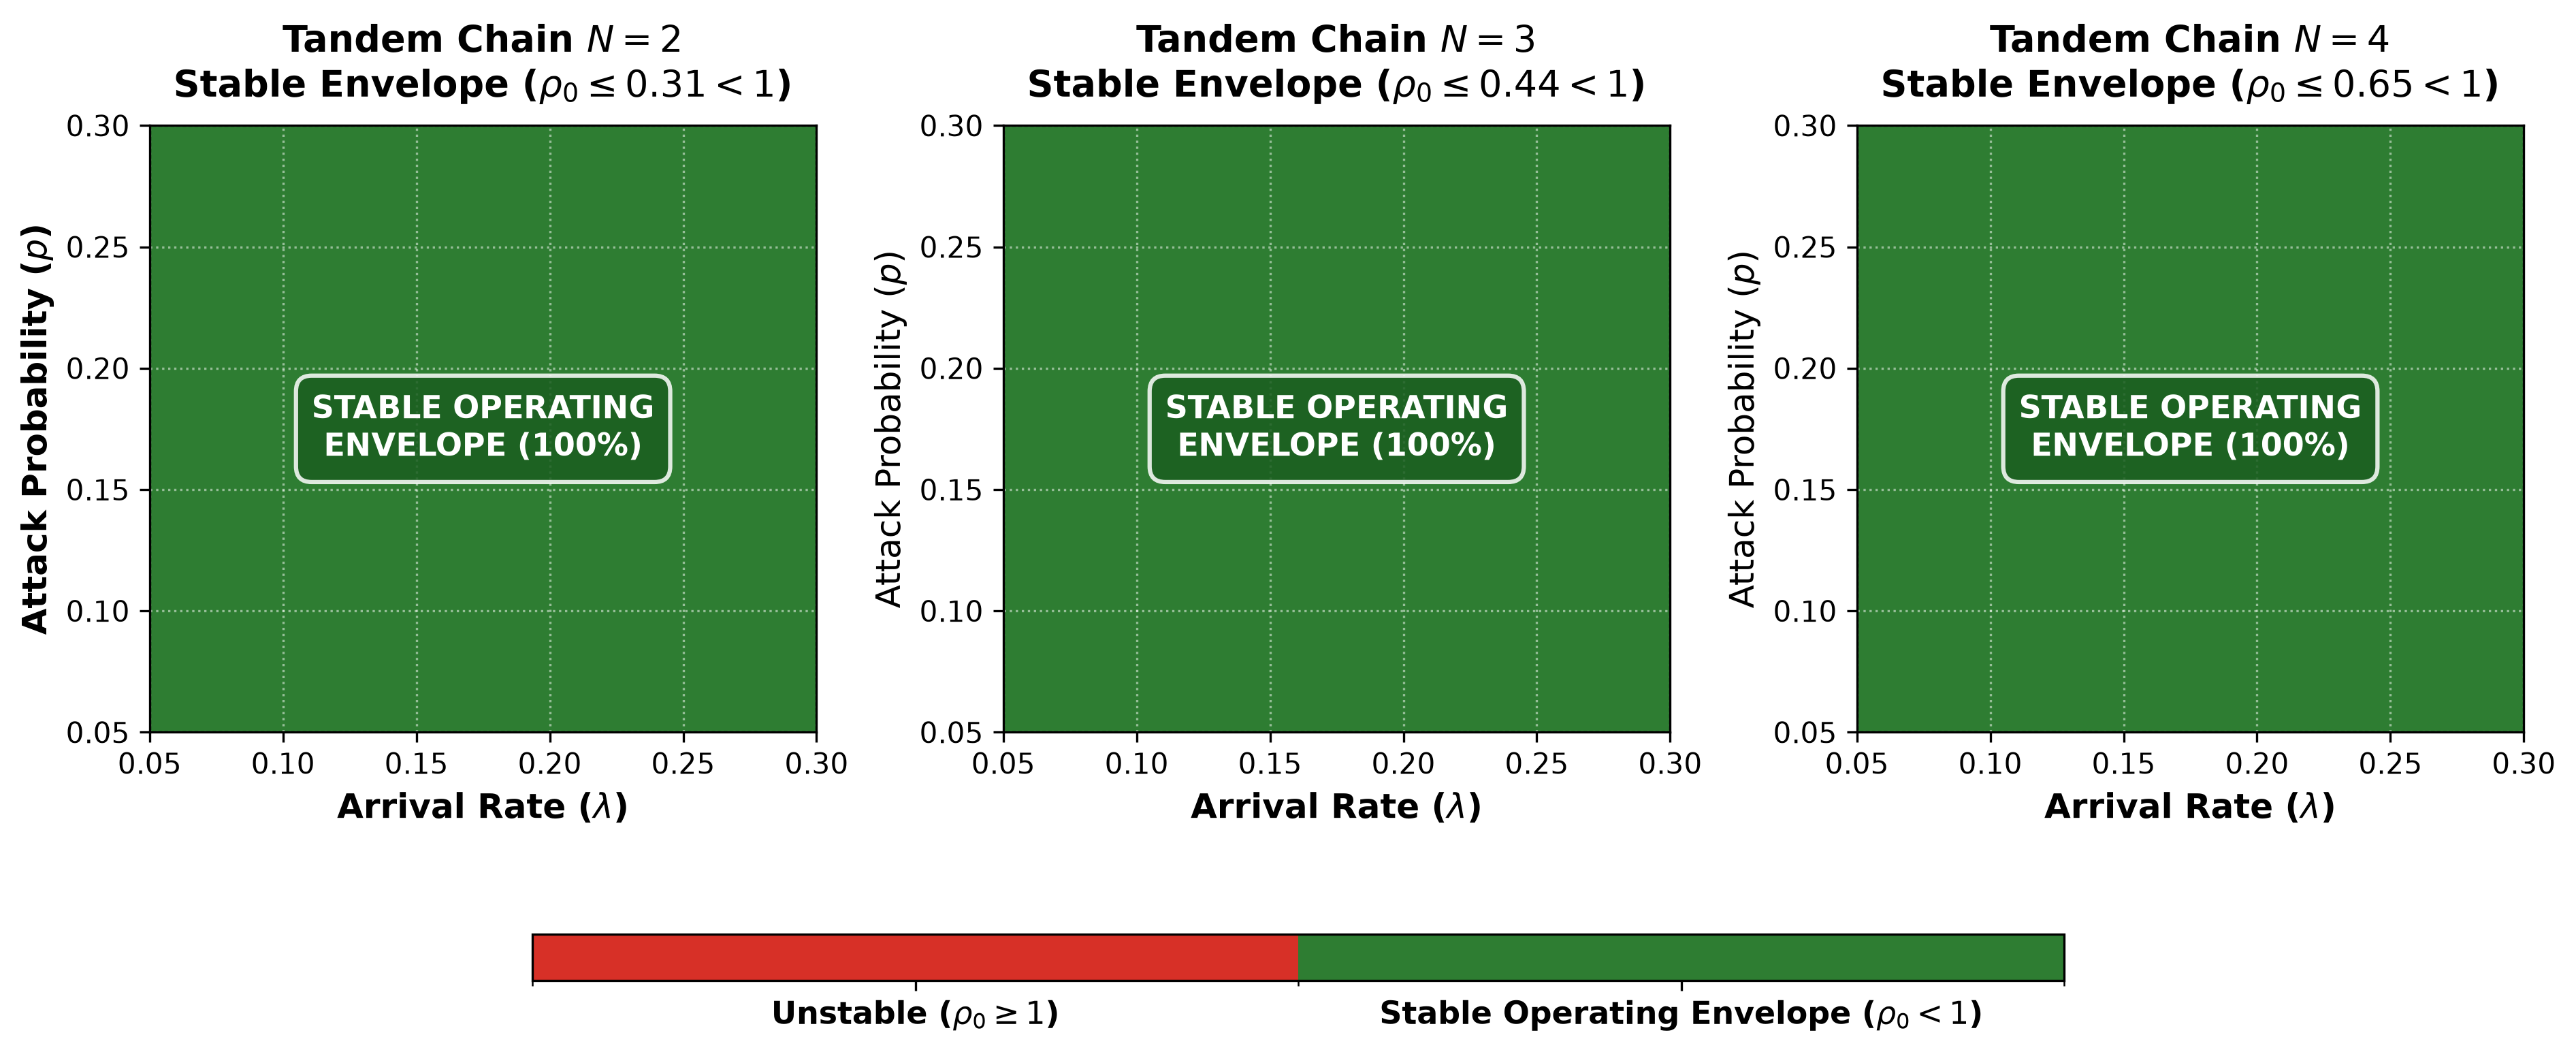
\includegraphics[width=\textwidth]{section_3_3_2_stability_regions.png}
        \caption{Stability envelope $(\lambda, p)$}
    \end{subfigure}
    \caption{Feedforward network dynamics (Cases 3 \& 4). (a) Super-linear delay growth with $N$ due to $(1-p)^N$ success decay. (b) 100\% stable operating envelope across $(\lambda, p \in [0.05, 0.30])$: bottleneck utilization satisfies $\rho_0 \le 0.65 < 1$ for all $N \in \{2, 3, 4\}$ under $\mu = 2.0$.}
    \label{fig:feedforward}
    \vspace{-3mm}
\end{figure}

\subsection{Delay Scaling and Stability Envelope}
Because all retransmissions re-enter at Node~0 ($\Lambda_0^* = \lambda / P_{\text{succ}}$), Node~0 represents the system bottleneck. As $N$ grows, $P_{\text{succ}}$ decays exponentially as $(1-p)^N$, driving super-linear delay growth (Fig.~\ref{fig:feedforward}(a)). 

Crucially, evaluating the stability condition $\rho_0 = \Lambda_0^*/\mu < 1$ across the operational grid $(\lambda, p \in [0.05, 0.30])$ under $\mu = 2.0, W = 8.0$ demonstrates that the system maintains a \textbf{100\% stable operating envelope} across all $N \in \{2, 3, 4\}$ (Fig.~\ref{fig:feedforward}(b)). Maximum bottleneck utilization is strictly bounded: $\max \rho_0 = 0.31$ for $N=2$, $\max \rho_0 = 0.44$ for $N=3$, and $\max \rho_0 = 0.65$ for $N=4$.

\section{Feedback Mesh Topologies (Case 5)}
Consider an interconnected network of $N$ symmetric queueing nodes with external Poisson arrivals at rate $\lambda$ per node (total rate $N\lambda$) and service rate $\mu$. Upon completing service at any node:
\begin{itemize}
    \setlength{\itemsep}{0.5pt}
    \item With probability $p$, the packet is attacked/corrupted, triggering an immediate failure and origin retransmission.
    \item With probability $1 - p$, the packet survives. If cumulative time exceeds $W$, it times out. Otherwise, with probability $q = \frac{1}{N+1}$ it exits successfully; with probability $\frac{N}{N+1}$ it transitions uniformly to any node ($r_{ij} = \frac{1}{N+1}$).
\end{itemize}

By Jackson symmetry \cite{jackson1957networks}, every node maintains the identical arrival rate $\Lambda^*$ and clearance rate $\gamma = \mu - \Lambda^*$. The duration of $k$ consecutive node visits follows an Erlang-$k$ distribution $S_k \sim \text{Erlang}(k, \gamma)$ with CDF $F_k(W) = 1 - \sum_{j=0}^{k-1} \frac{(\gamma W)^j e^{-\gamma W}}{j!}$ ($F_0(W) \equiv 1$).

Defining reach weights $u_k = (1-p)^{k-1} (\frac{N}{N+1})^{k-1} F_{k-1}(W)$, the expected server visits per attempt $E[V]$ and success probability $P_{\text{succ}}$ are:
\begin{equation}
E[V] = \sum_{k=1}^\infty u_k, \quad P_{\text{succ}} = \sum_{k=1}^\infty (1 - p)^k \frac{N^{k-1}}{(N+1)^k} F_k(W)
\label{eq:mesh_series}
\end{equation}
The fixed-point traffic balance at every node satisfies $\Lambda^* = \lambda \frac{E[V](\Lambda^*)}{P_{\text{succ}}(\Lambda^*)}$. Conditional durations are $E[D_{\text{succ}}] = P_{\text{succ}}^{-1} \sum_k P_{\text{succ}, k} \frac{k}{\gamma} \frac{F_{k+1}(W)}{F_k(W)}$ and $E[D_{\text{fail}}] = \frac{\sum_k (P_{\text{att}, k} + P_{\text{to}, k})\frac{k}{\gamma}}{\sum_k (P_{\text{att}, k} + P_{\text{to}, k})}$, where $P_{\text{att}, k} = u_k p$ and $P_{\text{to}, k} = u_k(1-p)[F_{k-1}(W) - F_k(W)]$.

\begin{figure}[t]
    \centering
    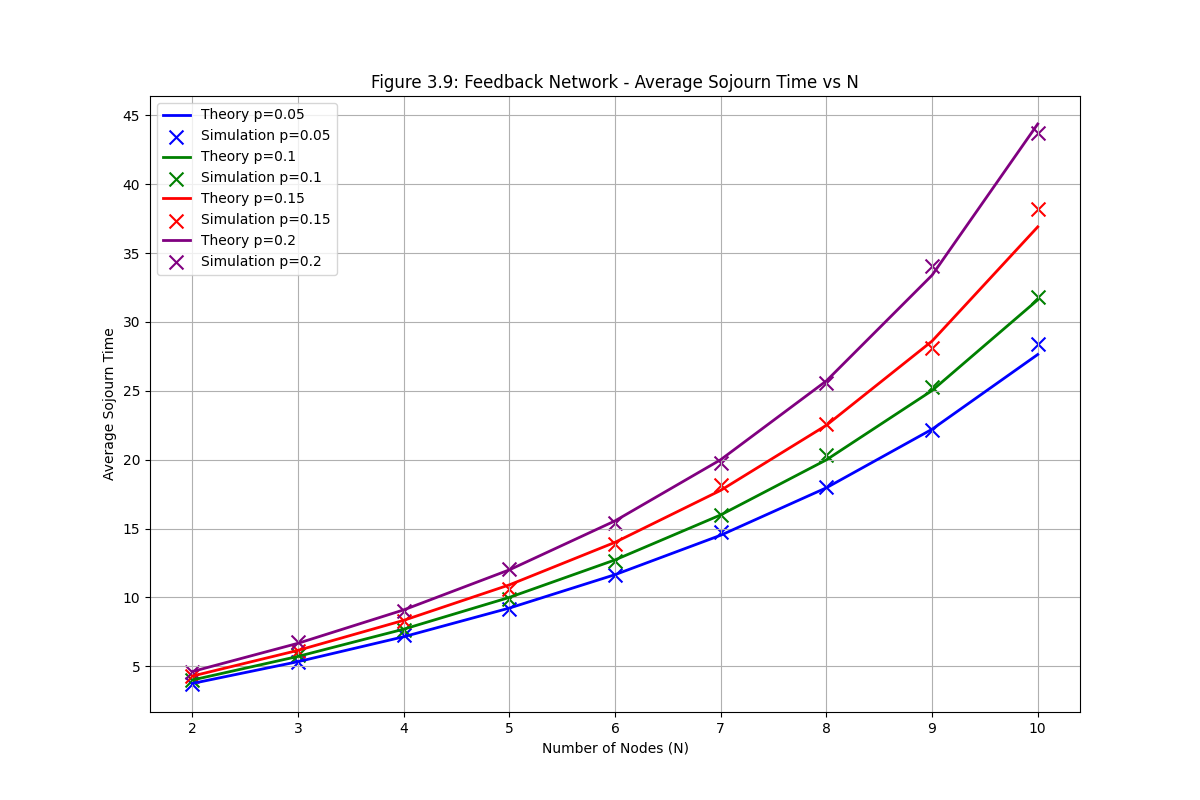
\includegraphics[width=0.30\textwidth]{section_3_3_1_sojourn_vs_N_varying_p.png}
    \caption{Case 5: End-to-end sojourn time in $N$-node feedback mesh networks. Uniform load-balancing across all $N$ nodes prevents localized bottlenecking, yielding resilient delay scaling.}
    \label{fig:feedback}
    \vspace{-3mm}
\end{figure}

\begin{table}[t]
\centering
\caption{Consolidated Analytical Models vs.\ SimPy Validation.}
\vspace{-1mm}
\resizebox{\columnwidth}{!}{%
\begin{tabular}{@{}lccccc@{}}
\toprule
\textbf{Case Study} & \textbf{Capacity $\Lambda_{\text{crit}}$} & \textbf{Theory (s)} & \textbf{Sim (s)} & \textbf{Abs.\ Gap} & \textbf{Error} \\ \midrule
1: Destruction & $\mu/(1-p)$ & 0.1286 & 0.1261 & 0.0025 & 1.91\% \\
2: Modification & $\mu$ & 0.1525 & 0.1523 & 0.0002 & 0.15\% \\
3: 3-Tandem & $\mu P_{\text{succ}}$ & 2.0511 & 2.0463 & 0.0048 & 0.23\% \\
4: $N$-Feedforward & $\mu$ & 2.9124 & 2.9079 & 0.0045 & 0.15\% \\
5: Feedback Mesh & $\mu$ & 31.606 & 31.804 & 0.1980 & 0.62\% \\ \bottomrule
\end{tabular}%
}
\label{tab:master}
\vspace{-2mm}
\end{table}

\textit{Structural Contrast with Tandem Chains:} In feedforward chains, Node~0 must process all retransmissions, creating an asymmetric bottleneck. In contrast, in symmetric meshes retransmissions re-enter the network and distribute uniformly across all $N$ servers. This load-balancing prevents localized queue explosion and yields resilient delay scaling (Fig.~\ref{fig:feedback} and Table~\ref{tab:master}).

\section{Experimental Validation}
The analytical models were validated against discrete-event simulations implemented in SimPy \cite{matloff2008introduction}, executing 30--200 independent replications with 5\,000--10\,000 time units per run after warmup. Table~\ref{tab:master} presents cross-validation across all five cases. Relative errors remain below 2\% in all cases, and strictly below 0.65\% across multi-node topologies. Specifically, under identical workloads ($\mu = 10, \lambda = 1.44, p = 0.2, W = 2$), modification attacks induce an 18.6\% delay surge over destruction ($0.1525$\,s vs.\ $0.1286$\,s), matching theory within 0.15\% error and validating Theorem~1. In 3-node and 4-node chains, Gamma moment-matching achieves exceptional accuracy (0.23\% and 0.15\% error). In the 10-node feedback mesh, theory aligns with simulation within 0.62\% error (the minor gap arises from truncating the infinite visit series at $k = 200$).

\section{Engineering Takeaways \& Design Guidelines}
The analytical framework yields three actionable design rules: (i)~\textbf{Timeout Tuning ($W$):} $W$ should be dimensioned to the $1 - \epsilon$ quantile of the unattacked journey distribution; smaller $W$ triggers premature retransmissions that exacerbate the feedback loop, while excessive $W$ delays failure recovery. (ii)~\textbf{Backoff Dampening ($B$):} While backoff adds delay linearly ($E[D] \propto B$), setting $B > 0$ paces re-injected attempts, dampening peak burst arrivals at bottleneck queues. (iii)~\textbf{Capacity Provisioning:} In feedforward chains, Node~0 must be provisioned with capacity $\mu_0 > \mu / (1-p)^N$ to absorb origin retries, whereas symmetric mesh networks distribute retries uniformly across all $N$ servers.

\section{Conclusion}
This letter formulated a unified stochastic framework for analyzing adversarial delay amplification across five network topologies under timeout-driven ARQ retransmissions. Three fundamental insights emerge: (i)~post-service modification attacks impose an exact $(1-p)^{-1}$ throughput penalty over pre-service destruction by consuming server cycles on corrupted attempts; (ii)~feedforward chains exhibit super-linear delay escalation due to geometric decay of path success, while maintaining a 100\% stable operating envelope across practical attack rates; and (iii)~symmetric feedback meshes distribute retransmission burden uniformly via Jackson symmetry, achieving resilient delay scaling. Future work will investigate adaptive timeout policies, multi-path routing, and non-Poisson bursty attack dynamics.

\section*{Acknowledgment}
The author gratefully acknowledges Professor Erol Gelenbe (Imperial College London and IITIS~PAN) for inspirational mentorship during the author's MSc thesis at Imperial College London, where foundational concepts of adversarial queueing were developed.

\begin{thebibliography}{99}
\fontsize{7pt}{8pt}\selectfont
\setlength{\itemsep}{0pt}
\setlength{\parsep}{0pt}
\bibitem{wood2002denial}
A.~D.~Wood and J.~A.~Stankovic, ``Denial of service in sensor networks,'' \textit{IEEE Computer}, vol.~35, no.~10, pp.~54--62, 2002.

\bibitem{pelechrinis2011denial}
K.~Pelechrinis, M.~Iliofotou, and S.~V.~Krishnamurthy, ``Denial of service attacks in wireless networks: The case of jammers,'' \textit{IEEE Commun.\ Surveys Tuts.}, vol.~13, no.~2, pp.~245--257, 2011.

\bibitem{gelenbe1991product}
E.~Gelenbe, ``Product-form queueing networks with negative and positive customers,'' \textit{J.\ Appl.\ Probab.}, vol.~28, no.~3, pp.~656--663, 1991.

\bibitem{gelenbe1993gnetworks}
E.~Gelenbe, ``G-networks with triggered customer movement,'' \textit{J.\ Appl.\ Probab.}, vol.~30, no.~3, pp.~742--748, 1993.

\bibitem{fall1996simulation}
K.~Fall and S.~Floyd, ``Simulation-based comparisons of Tahoe, Reno, and SACK TCP,'' \textit{ACM SIGCOMM Comput.\ Commun.\ Rev.}, vol.~26, no.~3, pp.~5--21, 1996.

\bibitem{jackson1957networks}
J.~R.~Jackson, ``Networks of waiting lines,'' \textit{Oper.\ Res.}, vol.~5, no.~4, pp.~518--521, 1957.

\bibitem{garetto2008modeling}
M.~Garetto, P.~Giaccone, and E.~Leonardi, ``Capacity scaling in delay tolerant networks with heterogeneous mobile nodes,'' \textit{ACM SIGMETRICS Perf.\ Eval.\ Rev.}, vol.~36, no.~1, pp.~13--24, 2008.

\bibitem{kleinrock1975queueing}
L.~Kleinrock, \textit{Queueing Systems, Vol.\ 1: Theory}.\hskip 1em plus 0.5em minus 0.4em Wiley-Interscience, 1975.

\bibitem{ross1996stochastic}
S.~M.~Ross, \textit{Stochastic Processes}, 2nd~ed.\hskip 1em plus 0.5em minus 0.4em John Wiley \& Sons, 1996.

\bibitem{altiok1985approximate}
T.~Altiok, ``On the phase-type approximations of general distributions,'' \textit{IIE Trans.}, vol.~17, no.~2, pp.~110--116, 1985.

\bibitem{cox1955use}
D.~R.~Cox, ``A use of complex probabilities in the theory of stochastic processes,'' \textit{Math.\ Proc.\ Cambridge Philos.\ Soc.}, vol.~51, no.~2, pp.~313--319, 1955.

\bibitem{burke1956output}
P.~J.~Burke, ``The output of a queuing system,'' \textit{Oper.\ Res.}, vol.~4, no.~6, pp.~699--704, 1956.

\bibitem{matloff2008introduction}
N.~Matloff, ``Introduction to discrete-event simulation and the SimPy language,'' Dept.\ Comput.\ Sci., UC Davis, Tech.\ Rep., 2008.
\end{thebibliography}

\end{document}
